\documentclass[11pt]{article}
\usepackage{multirow}
\usepackage[english]{babel}
\usepackage{multirow}
\usepackage{textcomp}
\usepackage{setspace}
\usepackage{caption}
\usepackage{subcaption}
\usepackage{times}
\usepackage{pdflscape}
% Set page size and margins
\usepackage[a4paper,top=2cm,bottom=2cm,left=3cm,right=3cm,marginparwidth=1.75cm]{geometry}
\usepackage{rotating}
% Useful packages
\usepackage{amsmath}
\usepackage{graphicx}
\usepackage[colorlinks=true, allcolors=blue]{hyperref}
\title{Decoding the sensation of pain from brain signals}
\author{Author: Thomas Sadler}
\date{\today}

\setstretch{1.2}
\begin{document}
\begin{titlepage}
   \begin{center}
       \vspace*{5cm}
       \Large
       \textbf{Decoding the sensation of pain from brain signals}

       \vspace{1.5cm}
       \normalsize
       \textbf{Thomas Sadler}

       \vspace{0.5cm}
       \normalsize
       \textbf{2101179}
       
                   
       \vspace{4cm}
       \normalsize
       A thesis submitted for the degree of Master of Science in Advanced Computer Science \\


       \vspace{2cm}
       \normalsize
       Supervisor: Dr Sebastian Halder \\
       School of Computer Science and Electronic Engineering \\
       University of Essex \\

       \vspace{0.5cm} 
       \normalsize
       August 2022 \\
            
   \end{center}
\end{titlepage}

\begin{abstract}

Pain is often defined as the most axiomatic symptom of medical conditions triggered by distinctive signals in your nervous system. Patients with mild Dysarthria find it extremely difficult to communicate with their doctors and often have the longest road to recovery as a result. This study aims to investigate a machine learning approach to classify EEG brain signals and interpret pain states simulated by various thermal stimuli. By cleaning the signal with independant component analysis and extracting power spectral densities from each frequency band, we are able to apply the data to three different classification pipelines each with a promising threshold of accuracy. The results of the investigation conclude that the Riemannian classification algorithm is by far the most impressive with a mean accuracy of 98\%. Followed by the common spatial patterns and source power comodulation algorithms boasting mean accuracies of 82\% and 75\% respectively. Furthermore, analysis of each frequency band confirm that the Beta and Gamma ranges are the most influential to our model's performance.
\newline
\newline
Keywords: EEG (Electroencephalogram), Python, MNE, MATLAB, PSD (Power Spectral Density)
\end{abstract}

\clearpage


\tableofcontents

\clearpage


\section{Introduction}

Everyday more and more illnesses develop that leave the afflicted vocally paralysed. These illnesses are majorly complicating medical staff's ability to communicate with their patients and diagnose just how much pain they really are in. Doctor's are currently having to rely on identifying ambiguous eye contact and body language to devise healthcare plans for patients without knowing the real root of the problem. This article investigates the ever-evolving field of brain-computer interfaces wherein brain signals are acquired from an abled participant and analyzed for characteristics that aid us to ascertain the pain index they are experiencing. Typically brain-computer interfaces contain two integral constituents: the brain, and an external device that acts as a communication pathway between the two. Although pain is inherintly counterfactual, data scientists are able to conduct controlled experiments in which we can simulate low levels of uncomfortability. Using a non-invasive electroencephalogram, we are able to collect the brain signals emitted from the participant whilst multiple "pain" stimuli are induced. Some of these acts involve either the participant submerging their hands under variable degree temperature water or certain occular events that help us distinguish between the two. The idea behind modern machine learning classification techniques is to memorize data and present outcomes based on the characteristics of that data. Classifying pain states is considered a supervised learning problem meaning we need to know which experimental event is being referred to by a specific segment of the data; this way we can train the model to perform as accurately as possible and generalize it's ability to predict the pain state of the participant. With the brain signals captured, the data must undergo a number of transformations to become a structure that can fit into one of these machine learning models, each of which requires a significant amount of modelling and analysis. 

The proceeding article will begin by outlining several accounts within the literature that provide some similar studies or alternative strategies within a similar context to this one. These summations will be descriptions of their methodologies, as well as an in-depth review of their results and how they may differ to the ones in this article. This chapter is designed to give those without the technical aptitude of a data scientists the ability to gain an adept understanding of  how others have approached a similar area of research without having to first understand the theory. The methodology is one of the most vital concepts that contributed to the success of this project. It is a combination of the overarching strategy of the research as well as a rationale of the steps taken to produce our conclusion. The initial chapters of this article will represent a summarised view of how the data was collected. The details of this will include, what the different experimental events were, what the environment was like, and what was used to capture the data over a select time period. 

The main body of the article is comprised of four subsections: Data analysis, Data Preprocessing, Feature Extraction and Data classification. Aside from the neuroscientific context of the project, the overarching scheme is still an artificial intelligence problem which all data scientists solve in the same way. First you clean the data by removing signals or frequencies affected by a noisy environment, then you extract the useful information from the dataset, ready to train the machine learning model. The trained model can subsequently be used to predict labels for the dataset with which it was provided. Each subsection of the main article will demonstrate an in-depth analysis of this process as well as justifications for all decisions made. The final section of this article will surmise the findings of the experiment. It will discuss the success of the Riemannian Classifier and how it outperforms that of the usual spatial filtering methods. Furthermore, it will investigate which regions of the scalp contribute the most to our models performance and which channels emit the most useful brain signals with respect to our experimental events.
 
Throughout the article, experimental events such as the participants eyes being open and closed are evaluated alongside that of pain states. It should be noted that evaluating occular activities is merely an initial test for our classification models. The main purpose of this study is to ascertain to what degree we can classify simulated pain states, not occular activity. The distinction between the two occular activites in comparison to the hot and warm water emersion is fairly obvious; if our models can succesfully predict these labels, we know that our pipeline is successful. 

\section{Literature Review}

2021 marked one of the largest inclines in international funding for brain computer interface studies, having tripled the \$97 million that was amassed in 2019. In a joint effort with increased funding, data scientists are continuously farming out new studies designed to help modernize the way that we tackle neurological medical issues. One of the most promising articles published last year was a study of acute pain detection from human EEG by Guanghao Sun Et al \cite{SUN2021108964}. By sourcing their data online they were able to amass the EEG data from approximately fifty one participants \cite{Tiemann2018-sm}. These participants, comprised of an equal number of men and women were recruited using local university bulletins with the requirements that any participant needed to be right handed. Guangaho Sun Et al. focused mainly on the motor condition of each participant on which 60 painful stimuli were applied to the left hand. The pain level was continuously varied between three indexes in a pseudorandomized sequence. The protocol is similar to the one carried out in this article, however instead of cutaenous laser stimulation inducing a "pinprick-like" sensation, each participants hands were submerged under variated temperature water. The EEG data was recorded using 65 electrodes and the 10-20 system, a popularly recognized method of applying the location of scalp electrodes in the context of an EEG exam. Sampled with a rate of 1000Hz and partially cleaned using a low pass and high pass filter the data was then downsampled to a rate of 500Hz and subject to the process of independant component analysis. This involved the authors manually identifying noisy components representing what could be interpreted as eye or muscle movement from MNE generated spatial topographic maps \cite{GramfortEtAl2013a}. This being considered as one of the major preprocessing steps of their project is similar to how the data was cleaned in this article; once the unrelated brain activity is identified and removed, it makes the distinguishing between experimental events all the more easier. After conducting source localization to find the most concentrated areas of brain activity from the cortical surface, the article proceeds to discuss and investigate their implementation of the state-space model and how it's optimized using the performance of one of eight possible regions of interest from two hemispheres of the brain. The results of the article were seemingly promising with seven trained models achieving a 0.7 or greater AUC statistic when used with "good" subjects. They were also able to surmise that given an appropropriately trained model, they could "achieve comparable results between cross-subject and within cross-subject prediction". The method adopted in this article when compared to commonly used batch supervised learning methods requires significantly less training trials whilst at the same time showing an increased mean peak area under the ROC curve thus demonstrating it's apt ability to predict class outcomes. Some of the observations made by Gaunghao Sun Et al. are impressively similar to the ones made in this article, most notably they noticed an increased in the theta and gamma frequency bands when comparing event-related potentials. Overall the paper was able to conclude with an approximate 70-86\% for detecting pain stimulus intensity with potential improvements to be made dependant on whether custom optimization is made for each subject. This article certainly lays the foundation for those looking to further investigate unsupervised machine learning methods to detect pain stimulus' in electroencephalogram data.  

Confusingly, previous articles have also shown promising results when using a significantly smaller number of channels when capturing the brain activity. In 2017, Jenessa Lancaster Et al used 16-channel EEG analysis, skin conductance and photoplethysmogram to detect cold pain stimulus using complex multivariate classificiation \cite{8008404}. The experiment in which they collected their data consisted of 60 trials, 20 of which involved three types of stimulus: cold pain, temperature control and an oculatory condition. The brain signals were measured across the sixteen channels in combination with the pulse and skin conductance using special sensors placed on the participants hands. Similarly to most EEG data comprised experiments, their data was analysed using Independant component analysis where movement, blink and alpha rythmic artifacts were treated as data contamination and removed altogether. Similarly to the pipeline used in this article, Jenessa Lancaster Et al epoched the data at 30-second intervals with all the following feature extraction methods acting on a single-trial level. After transforming the signal to the time-frequency domain using fourier transform \cite{bracewell1986fourier}, features were computed by calculating the root mean square signal amplitude of each channel. Providing these features with engineered physiological features to a sparse logistic regression model in combination with 10-fold cross validation, the company were able observe a significant increase in gamma activity in the frontal midline; a similar observation made to the results in this article. On average they were able to perform within a 79\% accuracy threshold whilst preserving some room to improve during future studies. By conducting some anaylsis of their predictions, they were able to conclude that the characteristics that led them to an increased accuracy presided more dominantly in the EEG data compared to the physiological data. Futhermore, Jenessa Lancaster Et al were able to confidently demonstrate that "pain responses can be reliably distinguised from general sensory stimulus responses"; an observation that can be validated from the work carried out in this article. These kind of results, that present a minimal amount of preprocessing steps are extremely promising precursors for real world implementation where signal noise, inconsistencies and participant unique pain thresholds are inevitable. They stated in their final comments that further studies into tonic pain, or chronic pain could be helpful tools for guiding data scientists feature selection methods and classification tuning techniques.

Another investigation in which cold tonic pain was used to classify pain indexes was by Rami Alazrai Et al in 2019 whereby they proposed a new approach that utilizes quadratic time-frequency distributions to construct time-frequency representations of EEG signals \cite{8941629}. The data captured in their experiment is extremely similar to the data supplied in this article. First the participants were sat down in a controlled environment then told to submerge their hand in water around 1.5-2.5 degrees celcius. The point at which the participants started to have an uncomfortable feeling was marked as the beginning of the pain state, this was continued until the feeling became unbearable at which point they could remove their hands from the water. Using the EPOC+ EEG system comprised of 14 electrodes in combination with the 10-20 placement system \cite{Herwig2003-xa}, the brain signals were captured at a rate of around 2048 samples per second. After passing the signals through a band-pass filter and down sampling to around 128 samples per second  Rami Alazrai Et al. utilized an inherently different system to the commonly used independant component analysis to remove noisy artifacts. Instead they used the automatic AAR (Automatic Artifact Removal) toolbox \cite{AAR} which doesn't require the authors to manually choose the least promising artifacts. The risk here is the toolbox automatically removing useful brain activity which may affect the accuracy of the classification models. Quadratic time-frequency distributions have already been proven in literature to detect certain phenomena such as oncoming seizures and certain evoked emotions. In this particular article Rami Alazrai Et al. used the QTFDs to transform the data from a one dimensional time domain signal, into a two dimensional time-frequency domain signal. As with all machine learning models, one of the most imperative steps with your training data is to reduce the feature dimensionality to better fit the model. This was done by extracting twelve particular time frequency features and then calculting values such as: Variance, skewness, kurtosis, mean, sum of logarithmic amplitudes and a few other minor statistics. Using these values as input for the support vector machine \cite{cortes1995support} in combination with a radial basis function (RBF) kernel, the group were able to amass a number of accuracy and f1 metrics in order to quantify how well their model was able to predict pain states. Impressively, Rami Alazrai Et al managed to average their accuracy out at around 83.4\% with the highest accuracy awarded being 93.46\% and the lowest being 73.61\%. Not only are the results obtained by the group comparable to the ones obtained in this paper, but the method is extraordinarily similiar. It can be argued that the work done in this article is an extension of that by Rami Alazrai Et al; using a multitude of classification models, with slightly more individualised features for each channel.

Some data scientists that commonly work with brain computer interfaces would argue that some of the most useful information in brain activity can be retrieved from a signals frequency bands. Potentially the most similar investigation to the one carried out in this article Pradkij Panavaranan et al. opted to use the power spectral densities of the Alpha and Beta frequency bands as their source for features to be supplied to a support vector machine model. Not only is their investigation similar to the one carried out in this article in the technical sense, but also in the way that the EEG data was collected; using heat as the pain stimulus. Nine healthy volunteers were chosen to participate in a non-invasive experiment in which they underwent a series of states, these are: 30 seconds resting phase, initiation phase in which the participant places their hands on a thermal pad heated to approximately 50-60 degrees celcius, pain phase in which they remain with their hands placed on the thermal pad for as long as can be tolerated and finally a concluding rest phase for 30 seconds. The EEG data was sampled at 512Hz using 32 channels placed using the 10/20 placement system. After having the raw data epoched,  Pradkij Panavaranan et al. split the signals frequency into it's Alpha (8-12Hz) and Beta (13-30Hz) constituents. Using a similar method to the other articles investigated in this paper, the band-split data was subject to the fast fourier transformation, meaning that the data was taken from the time domain to the frequency domain. The result is then used to calculate a list of power spectral densities; the proposed input to the pipelines fuzzy logic classification system. Although the pain index estimation was not proven to be effective, the classification accuracy was calculated to be effective up to 73.33\% of the time. That being said, the article goes on to argue that a polynomial support vector machine has significantly higher accuracy when predicting pain states than linear support vector machines with the accuracy averaging at around 96.67\%. The article also notes that making sure power spectral densities are normalized before they are supplied to the machine learning model is of paramount importance and almost always made for a significant increase in performance, especially when the feature space is highly dimensional. 

Not only is EEG brain activity analysed for pain detection purposes, but also for neurological stress symptoms that can't be recognized from the outside. Although this is a completely different objective to the one undertaken in this article, the pipeline starting from preprocessing the data to classfication of the features is similar in almost every aspect. In 2021, Dorota Kaminska et al. conducted an investigation into whether mental stress could be classified when induced from a virtual reality environment \cite{electronics10222840}. The initial data collection protocol involved inviting twenty eight healthy volunteers who adheered to the following critera: no neurological disorders, had previous use of VR without experiencing motion sickness, 20:20 vision. Note that the gender of the partipants were fairly skewed in favour of the male sex, however upon inspection of the articles results, it seems to have had no bearing on the outcome of the classification accuracy. In order to capture the brain signals, the participants had to wear not only an EPOC flex headset configured with 32 channels, but they also had to wear the virtual reality goggles in a manner that didn't affect the placement of the electrodes on the scalp. Similar to most pipelines that involve preprocessing the electroencephalogram data, Dorota Kaminska et al. opted to utilize independant component analysis available from MNE to identify and remove noisy artifacts such as eye movement, blinking, muscle movement and the heart's alpha rythm. The group followed by implementing further stages of preprocessing to the signal to improve it's general clarity. The first is a zero-phase finite impulse response filter; essentially a hamming window that slides across the signal and removes parts of the signal that do not adhere to the seven different customized parameters. The second was an epoch filter that filters the signal and rejects epochs where the peak-to-peak amplitude exceeds the reasonable limits for that specific type of channel. The group noticed that frequency bands with the most activity during a relaxation state were the Alpha and Theta bands. When the stress was induced to each participant, the Alpha and Beta bands underwent a significant change during the first minute however this was theorized by the participants to be due to an increase in concentration. Due to a blatent tampering of the feedback caused by the internal emotions of each participant, the group conducted stress classification individually under each frequency band leading to a large variety in results. It's stated the the best results, around 96.64\% accuracy, were achieved from theta-subset of features and the lowest results, around 76.85\% accuracy, were achieved from the beta-subset of features. The characteristics of these features are largely alike to the one used in this article. Although all frequency bands were used in classification as opposed to a single subset, pre-analysis of the data determined that the biggest presence of activity during the pain stimulus originiated from the theta frequency band and the lowest presence of activity during pain stimulus originated from the beta frequency band. Note that this correlation could imply a subtle association between classifying pain in EEG data and classifying stress. Aside from the features that led to their classification accuracies, the authors noticed that the support vector machine yielded the best results on almost every occasion. Judging by this investigation and most of the others in the literature available, SVM seems to preside over all models, no matter the classification problem being solved.

\section{Data Collection Protocol}

\subsection {Participants and Experiment}

The EEG data used in this article was sourced from Dr Sebastian Halder, a principal author of the article "Assessing the specificity of the relationship between brain alpha oscillations and tonic pain" in which it was also used \cite{VALENTINI2022119143}. It should be noted that according to Elia Valentini et al. the study was approved by the ethics comittee of the University of Essex. Having been sourced from 36 participants, the dataset used to train our model is comprised of brain signals recorded from twenty-two females, and fourteen males, each of which have a range of ethnicities. In line with most EEG recording experiments it was ensured that the participants adhered to a certain criteria before taking part, this includes: no visual difficulties, no neurological or psychiatric disorders and most importantly no pain disorders that could put their own safety at risk.

Pain being counterfactual, needs to be simulated to each of the participants in a non-invasive manor, this came in the form of thermal discomfort from variable temperature water. The experiment as a whole contains 5 unique experimental events of which the ocular actions occur twice:
\dots
\begin{itemize}
\item Submerging hands in “warm” water
\item Submerging hands in “hot” water
\item Non-painful auditory stimulation
\item Eyes Open
\item Eyes Closed
\end{itemize}

Each of the main three, non-ocular experimental events occured in randomized sequences however always between two resting phases. The first resting phase consisted of 2.5 minutes of the participants eyes being open and closed, with the final resting phase being the same thing. During both of the main experimental events, the participants were required to submerge their hands in a 30 litre tank of water. During the hot water submersion phase, the water was heated to approximately 45 degrees celcius. As cited in the original article, 45 degrees has been proven to inflict moderates amount of pain, regardless of the pain index of the participant. During the warm water submersion phase, the water was heated to approximately 6 degrees less than that of the hot water temperature. It was found that at 39 degrees, the participants felt no unpleasantness meaning that the data obtained from this phase could be effectively compared to the data from the hot water submersion phase. This procedure ensures the possibility of identifying characteristics of the signal and frequenices that were caused by the increased pain intensity. It was important during the experiment that the participants took note of how unpleasant the feeling was during the pain onset. This is because the final experimental event, the auditory stimulus, needed to be comparatively uncomfortable. By having the participants personally note their pain index caused by the hot water submersion, the authors were able aptly find a frequency that overcame any pain thresholds that could skew the data. For most participants, it was found that around 5000Hz frequency played through a pair of headphones was able to satisfy the requirement of an equally uncomfortable feeling to hot water pain stimulus. The sound stimuli event isn't investigated too extensively in this particular article however for Elia Valentini et al, it was required to "control for the negative affect contribution to the alpha oscillations". Note that the major experimental events took place for 5 minute intervals with small breaks inbetween.

\subsection{EEG Configurations}

The brain signals of each participant were measured using an electroencephalogram. An EEG is a tool often used by medical professionals to non-invasively record brain activity of patients using small metal disks known as electrodes. Typically electrodes are fitted by specially trained technicians using a special non-chemical adhesive, however when in possession of a special elastic cap designed to aid the placement of electrodes, the participant needs only to wear it with each electrode being pre-positioned on their scalp. Each of the small electrodes are connected via wires to a device that is designed to amplify each of the brain waves. When patients engage in any activity, or invoke some kind of emotion / feeling, the brain sends electrical impulses using synapse pathways. These electrical impulses are detected by the electrodes as abnormalities and recorded over time as one long signal in the form of a wave. Note that due to the sensitivity of electrodes when EEG recordings are taken, experiments require a fully controlled environment; inconsistencies such as eye movement, blinking, muscle movement and increased heart rate can cause distortion in the EEG readings, making it harder for a machine learning model to distinguish useful information from the useless. 

In the experiment in which the data used in this article was obtained \cite{VALENTINI2022119143}, 63 electrodes were mounted to each participant using the widely popular 10-20 system. The 10-20 system is a referencing guide for the locations of each electrode on the scalp. It is widely adopted in the BCI community due to it's consistent ability to effectively analyse all  brain communication impulses. The regions of the scalp covered by the 10-20 system are structured as follows. 

\begin{figure}[tb]
\centering
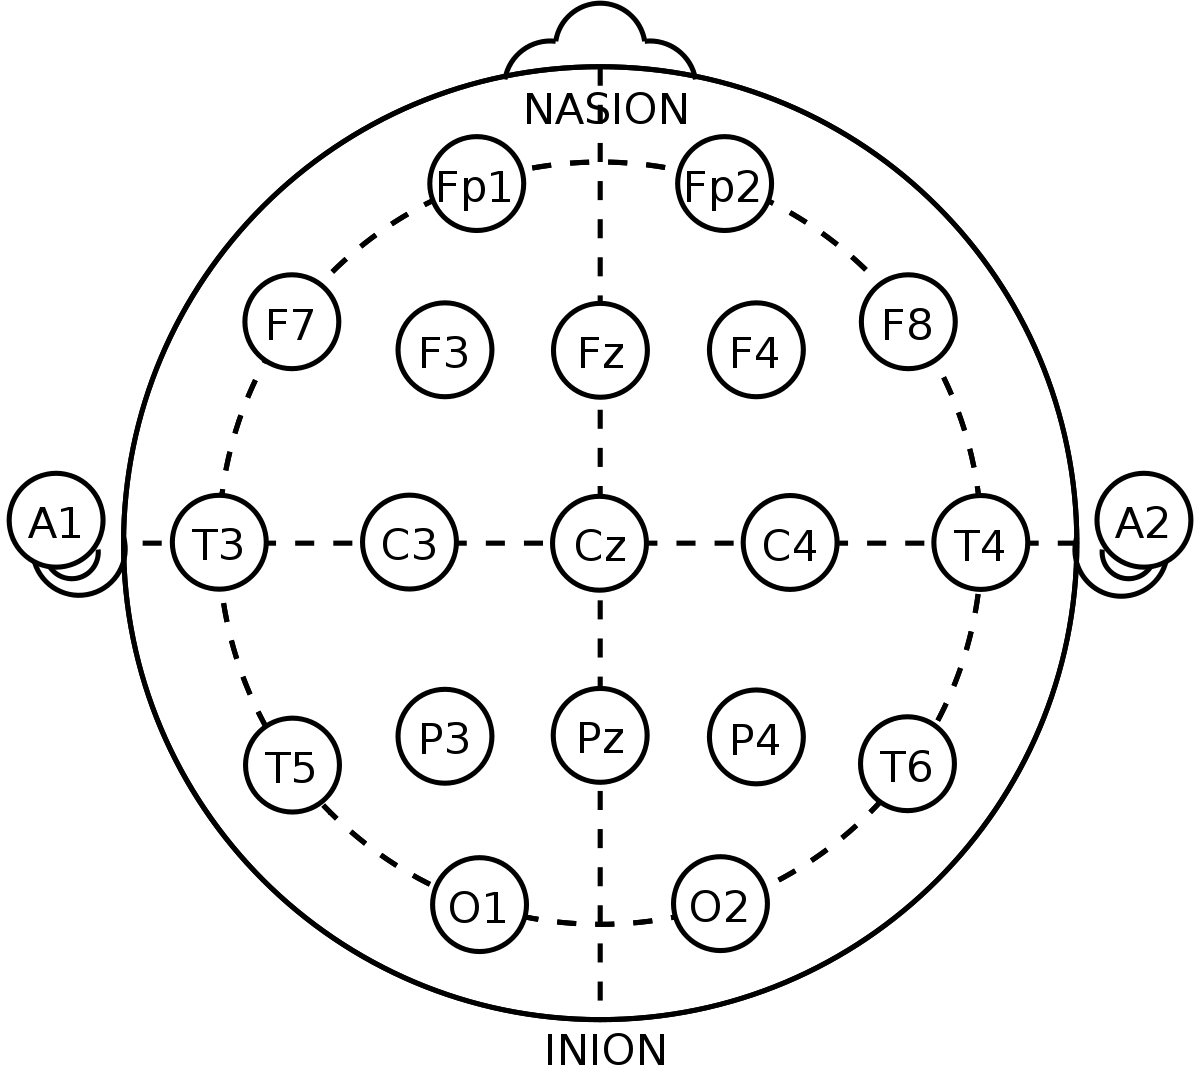
\includegraphics[width=0.5\textwidth]{ElectrodePlacementDiagram.png}
\caption{\label{fig:ECD}Labeled diagram of the 10-20 electrode placement system. These labels cover all regions of the brain and is popularly used due to it's consistency for measuring brain signals. Note this image, sourced from wikipedia, only has 21 electrodes visible. The electrode arrangement used to collect the data from this article has 63 electrodes, not 21.}
\end{figure} 

\dots
\begin{itemize}
\item F - Referring to the frontal portion of the scalp
\item P - Referring to the parietal portion of the scalp
\item T - Referring to the temporal portion of the scalp
\item O - Referring to the occipital portion of the scalp
\item A - Auricular
\item Odd numbers - Left side of the scalp
\item Even number - Right side of the scalp
\item Z - Midline of the scalp. 
\end{itemize}

These can be cross referenced with figure \ref{fig:ECD}, for those unfamiliar with which portions of the scalp the initial terms refer to. Note that A1 and A2 in the diagram (also known as M1 and M2) are contralateral referencing electrodes. 

\section{Data analysis}

\begin{figure}[tb]
\centering
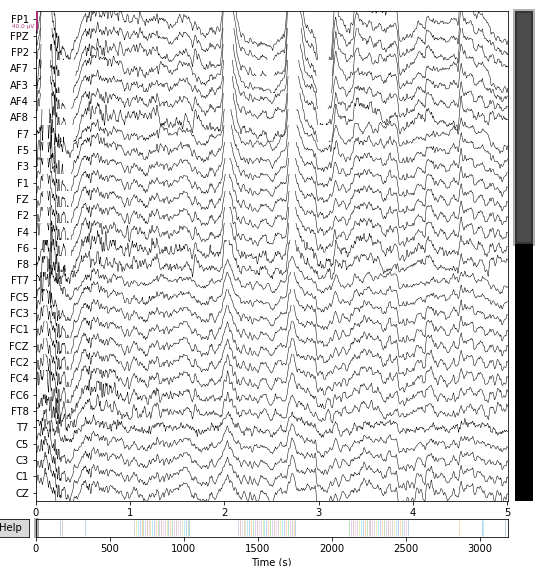
\includegraphics[width=0.8\textwidth]{RawPlot.png}
\caption{\label{fig:RawPlot} This figure depicts the raw signal plot of patient 3TM. Each horizontal line depicts the waveform of a single electrodes readings and can be cross-referenced with the labels along the y-axis. Noisy components are clearly indicated from the arbitrary sharp peaks at the 1400 and 1750s time periods.}
\end{figure} 


For the purpose of general clarity, this section of the article will investigate the analysis of a single subset of the data; this being the EEG data retrieved from a single participant, instead of every participant who engaged in the experiment. That being said, it should be noted that every subset of the data was treated with the same pre-processing steps. When the brain signals were measured, and the EEG output recorded, the results of the output were stored as Neuromag data. Neuromag data is stored in .fif files that can subsequently be used in FieldTrip; an open source toolbox that uses low-level MATLAB and MNE functions to load the data into a processable format \cite{Oostenveld2011-nu}. Using the necessary functions to load the .fif file, it was necessary to conduct a deep analysis of the raw data. We can begin by inspecting the most basic information regarding the data calculated for us by MNE. The raw data has approximately 101 events spanning from the beginning of the recording till the end. Only 95 of these events are unique and each of them have a unique label that we can cross reference with a fixed label dictionary to determine which event corresponds to which participant action. Using a similar practice, we can also surmise that the data was sampled using a frequency of 500Hz; an important value required to convert the data from samples to seconds. There is only so much information about the data that MNE will provide us with automatically. Most of the important observations need to be made manually using all the visualization techniques available. The simplest form in which we can visualize our data is as a raw object. Raw objects are modelled using the raw sensor traces contained within the data and are plotted across the time domain \ref{fig:RawPlot}. Each individual line extending horizontally across the graph, depicts the sample readings of a single electrode placed on the participants scalp and has a subsequent label ascending the y-axis to aid with corresponding between the two. Alongside the graph itself, we are provided with a time legend that clearly depicts each of the seven experimental events \ref{fig:Epoch}. For this particular experiment, we can see the participant began with the inital eyes open and eyes closed ocular events, followed by the three main pain stimulus events, with another final occular resting phase to conclude. Given the nature of the project, it's clear that only the information stored within these 7 time frames are useful for training our machine learning models. Rather than manually excluding the resting phases between each experimental event, it would be easier to simply epoch our experimental events using calculated time markers. Initial inspection of the raw graph indicates some clear noisy components visualized as strong unnatural peaks in the sample readings. The most obvious examples of these can be observed around the 1400s / 1750s time period. These artifacts could take the form of unwanted brain activity caused by muscular and occular responses from the participant that may interfere with the extraction of our wave features. Aside from these sharp peaks, there are no clear signs of noise with most electrode samples conforming to a similar shape. 

\begin{figure}[tb]
\centering
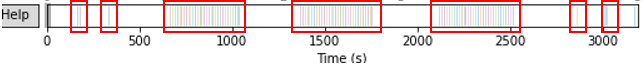
\includegraphics[width=0.8\textwidth]{Epoch.png}
\caption{\label{fig:Epoch}The legend using in combination with the raw data plot depicting the time scale in which each of our experimental events happen. Using some simple red boxes we can clearly identify the 4 smaller resting phases as well as the 3 main pain stimuli. Each of these sectioned phases continue to be epoched in the later stages of the pipeline. This figure was modelled using the MNE plot function.}
\end{figure} 

Another more useful method in which the data was visualized was using a power spectral density plot \ref{fig:PSDPlot}. Power spectral density plots (PSDs) are a measure of a signals power against their frequency. Similar to the raw plot, PSDs have their own coloured topographical legend that aids users to identify which readings on the plot correspond with which part of the participants scalp. Immediate inspection of this graph doesn't indicate too many principal characteristics that are of use later in the pipeline, more so useful observations that are worth taking note of. The first of these observations is a clear broken electrode located somewhere in the occipital / left temporal region of the scalp. This is shown on the plot as an out of place line that doesn't conform to the same pattern as the rest of the readings. Although this was initially ignored in the analysis stage of the project, there were a number of alarming outputs made during the data's feature extraction that would affect the validity of our model accuracies. By performing some event analysis in which we plotted the differences in frequencies between two experimental events for each channel, it was determined that one of our channels displayed atypical levels of differences compared to the rest of the electrodes. This electrode was discovered to be T7. Although T7 is not confirmed by Elia Valentini et al. to be the broken electrode, results from classification indicate clear improvements when all the data from T7 is removed from the dataset. Another observation made from the power spectral density plot is a slight peak at around 50Hz. This peak does not pertain to any activity taken place within the brain but instead from the electricity grid. In the UK, alternating current oscillates 50 times every second meaning most electrical equipment and appliances are designed to work at 50Hz. This interference does have an effect on the EEG readings in a vizual sense however does not affect the useful information which is captured at lower frequencies. Were interesting brain activity to take place at the 50Hz frequency band, the experiment would need to take place inside a shielded room, without the presence of any electrical devices.

\begin{figure}[tb]
\centering
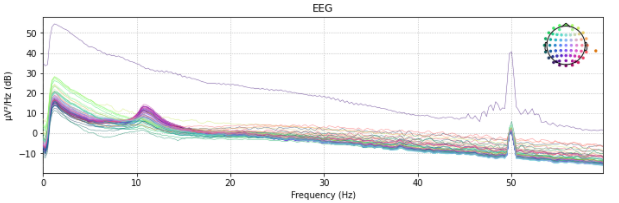
\includegraphics[width=0.95\textwidth]{PSDPlot.png}
\caption{\label{fig:PSDPlot}
Power Spectral density plot measuring the signal power against frequency of the first patient in the EEG dataset. Using the coloured topographical legend, we can cross reference each line on the plot (each electrode) to a particular placement on the scalp. As noted above, the line seperated from the plots main tendency has been recorded as a broken electrode and is theorised to be channel T7. Furthermore the mound residing at the 50Hz mark is a result of the electricity grid as opposed to any useful brain activity sourced from the participant.}
\end{figure} 

\section{Data Preprocessing}

\subsection{Frequency Filtering}

Frequency filtering is an extremely useful process used to filter signals according to preset frequency parameters. It has been proven in literature to increase the signal-to-noise ratio (SNR) however requires delicate implementation so as to not warp your data \cite{Filtering}. Filters are typically broken into two complicit classes, the one implemented and focused on in the proceeding article is the finite impulse response filter (FIR). Finite impulse response filters are typically easier to control and have a well-defined passband. Furthermore they are proven to be more stable then their counterpart IIR and can easily be converted to minimum-phase. The filter implemented in this project was a slow drift filter. The term "slow drift" refers to a gradual change in output value without any internal change. Typically this filter is used before implementing independant component analysis. Upwards slow drifts, over time, can make independant artifacts appear less independant which will in turn make the ICA filter's time of finding an accurate solution to the signal more difficult. High-pass filters are recommended to combat this problem, therefore a high-pass filter with a cut-off frequency of 1Hz was used. 


\subsection{Independant Component Analysis}

Independant component analysis, the second stage of signal pre-processing, is a widely utilized machine learning technique that focuses on seperating independant sources from a mixed signal \cite{Li2017AutomatedEA}. A popularly used metaphor for this is the instrument scenario. Imagine three different instruments are playing in the same room, and three seperate microphones are recording the sound signals; ICA can be used to isolate these three sources. In our case, the 63 different channels represent the microphones that are continuously recording the "instruments" which are interpreted as useful brain signals, ocular activity, muscular acitivity, alpha rythm etc. The process of independant componenent analysis is typically as folllows. First the data is scaled to unit variance and whitenened using principal component analysis. The result from these two steps are then passed to the ICA algorithm whilst specifying the number of artifacts to detect. Unfortunately independant component analysis is fairly computationally expensive, therefore efficiency of attempting to detect a higher numbers of artifacts is completely dependant on the computational power of your own hardware system. As with most hardware intense machine learning processes, the positive trade-off is that the more artifacts isolated, the more accurate the signal will be after the recognizable noisy artifacts are removed. In the context of our project, 30 components were isolated from each participants signal readings. Once each of the artifacts are isolated, they must be manually inspected in order to be recognized as "useless" signal activity. Note that there are automatic methods to remove noisy signal artifacts such as the popular AAR toolbox offered by MATLAB \cite{INDCA}, however risking useful brain activity being removed from the data could be detrimental to the final models classification accuracy. When the artifacts are visualized using scalp topographies, power spectral density plots and ERP charts, they are plotted in order of their variance in the data. Although the 25th isolated artifact might look really bad from the visual indicators, chances are is has almost no affect on the data. Given that there are 36 particpants in the dataset, it was decided that only the top ten of these thirty artifacts would be inspected for unwanted behaviour in order to preserve the amount of time taken during the preprocessing stage. Removing any higher than the tenth artifact would result in almost no difference to the signal therefore wasn't worth the time it would take to do so. Note that looking at the first 5-10 artifacts in independant component analysis is common practice in brain computer interface projects as stated by Md. Kafiul Islam Et al \cite{inbook}.

 \begin{figure}[tb]
\centering
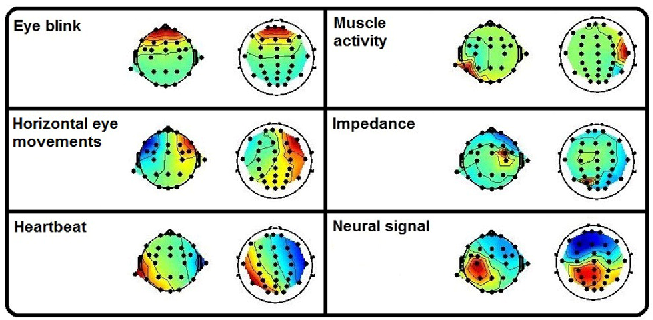
\includegraphics[width=0.95\textwidth]{Noise.png}
\caption{\label{fig:Noise}
This figure depicts examples of scalp topographies for six unique noisy artifacts, triggered by activity that was not conducted by the brain. Most of the artifacts can be identified by a range of  means however eye blinks have a clear anterior weight distribution on the scalp making them the easiest to identify. This image was taken from the article "Automated EEG artifact elimination by applying machine learning algorithms to ICA-based features", composed by Yandong Li Et al. \cite{Li2017AutomatedEA}}
\end{figure} 

There are typically four major noise components to look out for when analysing isolated artifacts. The first is occular activity. Typically the most obvious of the unwanted artifacts, occular activity such as blinks or general eye movement can usually be identified by an obvious anterior distribution of weights towards the frontal portion of the scalp. You can also identify individual blinks using the ERP representation where they make take the form of small, seperated dots in a clear chart. The second noisy artifact that has the highest variance in the data is muscular acitivity. Muscular acitivty can usually be recognized by immediate high peaks in the activity power spectrum just before the usual 1/f shape, triggered by sudden arm or leg movements. It is fairly difficult to recognize muscular activity on a scalp topography therefore is recognized as one of the hardest artifacts to accurately identify and remove. As previously stated, due to the impact that removing useful brain signals can have, it is always better to ignore indistinct artifacts and have some extra noise to contend with. The third category of artifacts that should be removed are those whose ERP graph's potray the hearts alpha rythm. Note this should be cross checked with the scalp topography that's weights should be posteriorly dominated. Given the fact that we only want to be analysing data depicted as brain activity, it seems illogical to keep heart activity in the signal. The final category of artifact to be removed in line interference. Similar to muscular activity, line interference can be identified using the activity power spectrum. Line activity is often characterised by a large arbitrary peak at the 50Hz marker. As previously disclosed in the article, peaks at the 50Hz marker will almost always be caused by nearby electrical devices that are calebrated to operate at 50Hz.

For most datasets in this project, anywhere between 0-4 artifacts were removed at any one time. It should be fairly obvious whether removing a specific artifact has had an affect on the raw data simply by plotting the original against the cleaned signal \ref{fig:ICA_Comp}. 

 \begin{figure}[tb]
\centering
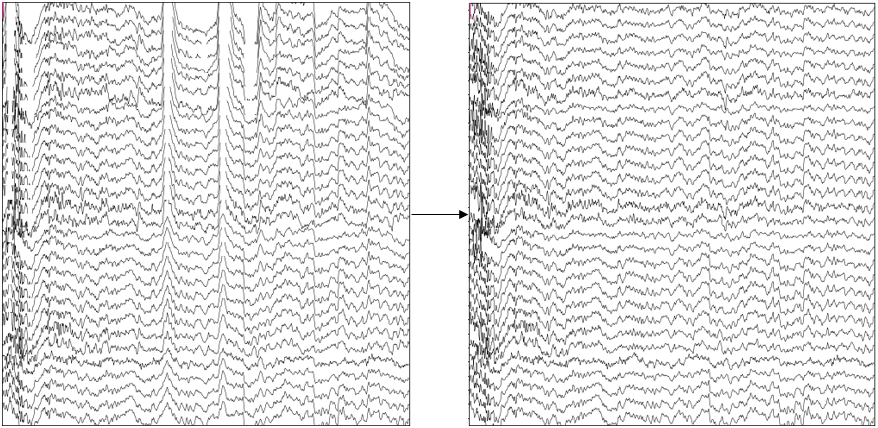
\includegraphics[width=0.95\textwidth]{ICA_Comparison.png}
\caption{\label{fig:ICA_Comp}
Raw plot of the first partipant alongside the raw plot after independant component analysis has occured. We can clearly observe that removing certain artifacts has removed large, arbitrary peaks and pits from the original signal. The signal lines now potray a more uniform line with clear brain activity occuring. These images were sourced from the program script used for this article wherein the first participants data has been pre-processed and classified.}
\end{figure} 

\subsection{Epoching}

Before extracting our features it's imperative that the signal be epoched into it's seperate experimental events. Epoching is essentially a procedure in which specified time-windows are extracted from a continuous electroencephalogram signal. Each of these segmented time windows are referred to as "epochs" or "trials" and typically concentrate on a unique event. Conducting this procedure ensures that when we extract our power spectral densities, we can keep track of which features correspond to which experimental event. This also gives us the ability to compare epoch features and evaluate the size of the difference between two given experimental events in particular frequency bands. In order to investigate the procedure of epoching, one must first grasp the concept of signal events. Events in signal processing are recorded as electrical signals which in the signal itself can be recognised by brief DC shifts or squarewave pulses. These events are typically used to mark the onset of experimental events. Most modern datasets record events using a series of "STIM" channels however the dataset used in this article hasn't marked stimulus onsets as "events" but instead as annotations. Generally speaking both events and annotations do the same thing which is analytically "describing" what happened during a specific time index. Luckily MNE provides a useful algorithm that automatically reads annotations marked in the signal and converts them to an event array. Events typically come with a unique ID corresponding to the experimental event they belong to, which for our dataset can be decoded as follows. 
\dots
\begin{itemize}
\item Eyes Closed; EEG Marker 4
\item Eyes Open; EEG Marker 5
\item Hot Temperature Submersion; EEG Markers 11-40
\item Warm Temperature Submersion; EEG Markers 41-70
\item Sound Stimuli; EEG Markers 71-100
\item Eyes Open; EEG Marker 7
\item Eyes Closed; EEG Marker 6
\end{itemize}

By utilizing the fully numpy array of sequential events, we can use their corresponding labels to distinguish the exact start and finish times of each experimental event. Note that once annotations are converted to events data structures using MNE, each events occurence in the signal is recorded by it's sample time instead of the time in seconds. Each of the events had to be converted from samples to seconds before being used to epoch the experimental events from the raw signal. Given the EEG recordings were sampled at 500Hz, the sample time must be divided by this value in order to obtain it's occurence in seconds. Once each of the experimental events have been epoched from the raw signal, we essentially have seven continuous epochs. The data contained in each of these epochs is completely unique to the experimental events that it corresponds to. The final step before analysing potential features, is to epoch the epochs again. Currently our seven epochs are continuous and when fed to a machine learning model would be read as a single row of data. The epochs require a further breaking down into fixed length epochs that are segmented using regular 10 second intervals. These new epoch data structures are shaped as follows: Trials x Channels x Samples. With seven unique epochs containing multiple trials each, characteristics of each experimental event can be investigated and visualized, resulting in an estimation as to how our models will perform. 


\section{Feature Extraction}

\subsection{Event Analysis}

Feature extraction is argued amongst data scientists to be one the most vital procedures in brain signal interfaces and signal classification. Feature extraction refers to the transformation of raw data into a set of numerical values that can be used to characterise the data from which it came. The data is then evaluated and fed to a machine learning model which uses these features to predict the outcomes of new, unlabelled data. Often neglected in electroecephalogram signals, power spectral densities of a signal can be one of the most useful features to train machine learning models due to their consistent individuality. In 2012, Yili Li Et al. conducted an investigation into the classification of EEG signals using a combination of both power spectral densities and riemmannian geometry \cite{features}. They found the results of the investigation to be compelling, with their results being "superior to commonly used metrics of K-L divergence". In order to observe how well power spectral densities will perform when training our models, we can conduct some preliminary research and investigate how different the signals are, inside of the frequency domain. In order to make sense of frequency domain plots, we must first know the different frequency bands in a signal is and what they mean. A frequency band is essentially a frequency interval inside a signal parameterised by upper and lower frequency bounds. Below are the five different frequency bands being investigated in this article. 
\dots
\begin{itemize}
\item Delta Band 0.5Hz - 4Hz
\item Theta Band 4Hz - 8Hz
\item Alpha Band 8Hz - 12Hz
\item Beta Band 12Hz - 30Hz
\item Gamma Band 35Hz+
\end{itemize}

	Note that the specific bounds these bands reside in are often argued by data scientists, however according to literature, these are the most frequently used. Activity inside frequency bands is highly investigated in the brain computer interface community with many characteristics of each correlating to human actions. For example in 2022, Hohaia W. Et al. investigated the alpha frequency band, specifically in the occipital region when the eyes are closed \cite{city27825}. The result of this investigation concluded that when the eyes are closed, we typically observe an increase Alpha compared to when the eyes are open. By extracting the power spectral densities from our epoched data, and plotting it using some simple line graphs, we observe some extremely decisive shaping which seems to corroborate the conclusion made by Hohaia W Et al \ref{fig:Chart}. 

\begin{figure}[tb]
\centering
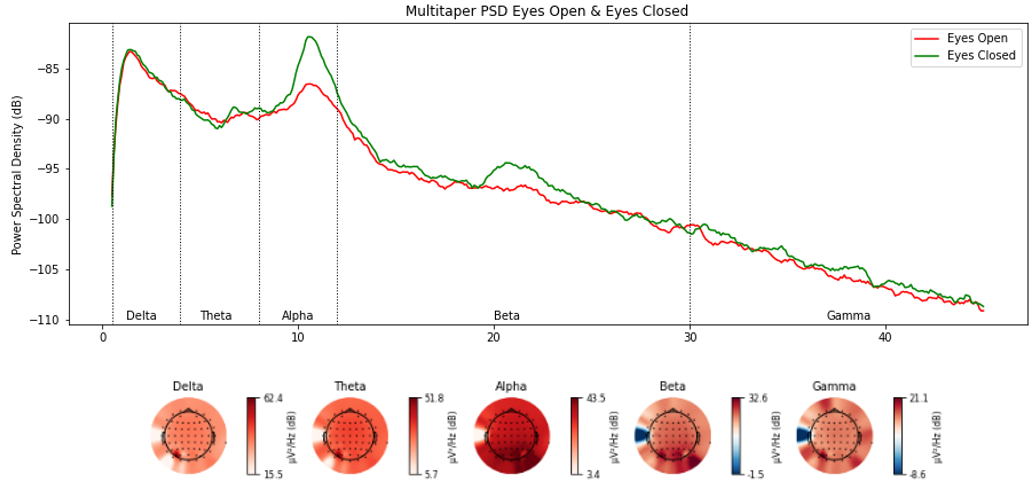
\includegraphics[width=0.95\textwidth]{2.png}
\caption{\label{fig:Chart}
Line graph constructed using the power spectral densities of the eyes open and eyes closed experimental event. Clearly we can see an obvious increase in the Alpha frequency band as well as some slight increases in the Beta frequency band which seems to line up with the literature. This graph confirms that it should be relatively simple for our machine learning model to distinguish between the two. }
\end{figure} 

Given the degree of difference between the eyes open and eyes closed event inside the Alpha frequency band, it should be fairly trivial for the machine learning model to distinguish between the two. Alongside the characteristics of each frequency band, we can also use the topographical weight distributions to confirm what our data is showing. For example, when performing certain occipital activity, we should typically see a increased distribution of topography weights towards the occibital lobe of the partipant. Although it is fairly simple to distinguish between occular activies in signal readings, it is much harder to distinguish between pain and non-pain states. We expect the differences between hot water emersion and warm water emersion to be much more subtle which will in turn make it more difficult for the machine learning model to predict their labels. By plotting the power spectral densities of our warm and hot water epochs using the same procecdure used for our occular events, we can see there is no clear distinction between the two \ref{fig:Chart_Pain}. This confirms the theory that pain states will be much harder for our models to identify and we should expect a fairly large decrease in prediction accuracy when compared to our occular events. Although arguable, the only slight characteristics we can see from our visualizations is the subtle decrease in the Beta and Gamma frequency bands during the pain state. Given the degree of difference between the two sets of power spectral densities in the Beta and Gamma range, it's unlikely that they will have a large effect on how the data is classified. The frequency band topographies also indicate no obvious distinctions between the two events. Although plotting these values has confirmed that predicting pain states will be more difficult than predicting occular actions, it also confirms that power spectral densities could be a promising feature to investigate more, especially with the machine learning models we have chosen to utilize.

\begin{figure}[tb]
\centering
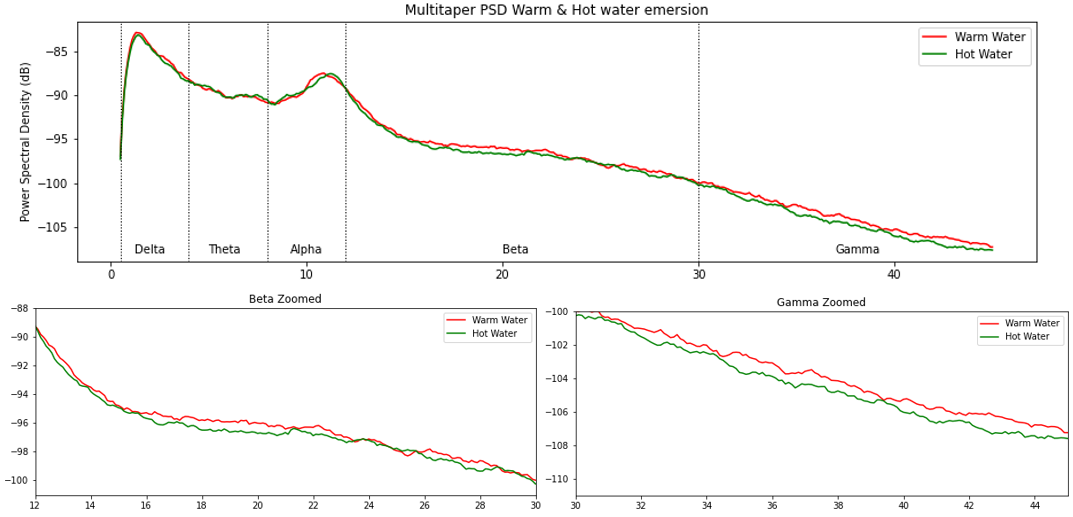
\includegraphics[width=0.95\textwidth]{1.png}
\caption{\label{fig:Chart_Pain}
Line graph constructed using the power spectral densities of the warm water emersion and hot water emersion experimental event. There is no clear difference between any of the frequency bands during theses states apart from an extremely subtle decrease in both the Beta and Gamma bands. This graph confirms that we should expect lower prediction accuracies in comparison to our occular events.}
\end{figure} 

\subsection{Predicted Regions of Interest}

Viewing the discrepencies between between frequency bands isn't the only way we can analyze and predict how the models will perform under certain parameters. We can also look more specifically into the individual channels that are the most likely to distribute the most useful training data. Looking at channels individually as opposed to their averaged value is useful when classifying between specific simulated pain states. Bearing in mind there are 63 channels in total, it's likely that some channels will contain more beneficial information than others which may just contain noisy data. The overarching goal here is not only to reduce our feature space enough for our training models to cope better with the training process but also to predict where feature selection models such as common spatial patterns and SPoC are most likely to extract their training information from. Areas of the scalp where channels are more proficient than others are also referred to as "Regions of Interest". ROIs contribute to the bulk of the models training accuracy in most cases, and the more we can isolate them, the better our models will be able to predict new labels.

Given our main feature set are power spectral densities, it seems fitting to use the initial results to calculate our regions of interest. This is done by extracting and calculating the mean power spectral densities from two different experimental events per channel and subtracting the corresponding values from eachother. This procedure results in a number of channel difference values that give abstract overview of which channels are the most likely to selected by our feature selection models. It should be noted that during this section of the project, the difference value of the channel T7 was unusually large given the rest of the results and was therefore treated as an outlier. Furthermore, the placement of T7 on each participants scalp positively correlates to the previous power spectral density graph where our broken electrode can be observed on the left temporal portion of the scalp. It is for these reasons that T7 is assumed to be our broken electrode and was removed from the dataset to avoid any skewed accuracies.

Below is a table depicting, in descending order, which channels represented the largest difference values in each frequency band, and are likely to contain the most useful training data.These are effectively our regions of interest.

\begin{center}
\begin{tabular}{ ccc} 
\hline
 & Eyes Open vs Eyes Closed & Warm Water vs Hot Water\\
\hline
\multirow{1.2}{5em}{Delta}
& F4, AF4, FC4, F2, F6, FC2 & AF8, AF7, FP2, FP1, O2, OZ\\ 
& FC6, FZ, AF3, FC3  & O1, PO8, PO6, PO7 \\
\multirow{1.2}{5em}{Theta}
& FC4, F4, FC2, AF4, FCZ & PO6, AF8, O1, FT8, P7, PO7 \\ 
& F2, PO4, F6, PO7, P6 &  FT7, O2, PO8, OZ \\
\multirow{1.2}{5em}{Alpha}
& POZ, PO4, O2, PO8, OZ, PO3  & PO6, PO7, O1, P7, PO8, P5 \\ 
& O1, PO7, P6, P8 & FT7, OZ, PO3, O2 \\
\multirow{1.2}{5em}{Beta}
& O2, PO4, POZ, OZ, PO3, O1  & TP7, PO6, T8, FP1, FT8, PO7\\ 
& PO8, PO7, P6, P5 & C5, FT7, O1, P8 \\
\multirow{1.2}{5em}{Gamma}
& T8, O2, PO4, POZ, OZ, PO3  & TP7, PO6, P8, FT7, F5, FP1 \\ 
& O1, PO8, F5, P5 & FT8, C5, T8, PO7 \\
\hline
\end{tabular}
\end{center}

During feature extraction, it's not possible to calculate power spectral densities for specific frequency bands. If this were done our result wouldn't reflect accurate regions of interest for the dataset as a whole but instead partial sections of the frequency spectrum. For this reason, using the values from the table, regions of interest must be created that accomodate the most effective channels from all frequency bands. This was done by conforming the top 8 most effective channels from each frequency band into one list. Doing this has not only dramatically reduce the dimensionality of the feature space, but also given the ability to visualize where we expect the CSPs and SPoC to choose the most useful channels from. MNE provides a built in algorithm for visualizing scalp topographies with respect to a strict set of channels \ref{fig:ROI}.

\begin{figure}[tb]
\centering
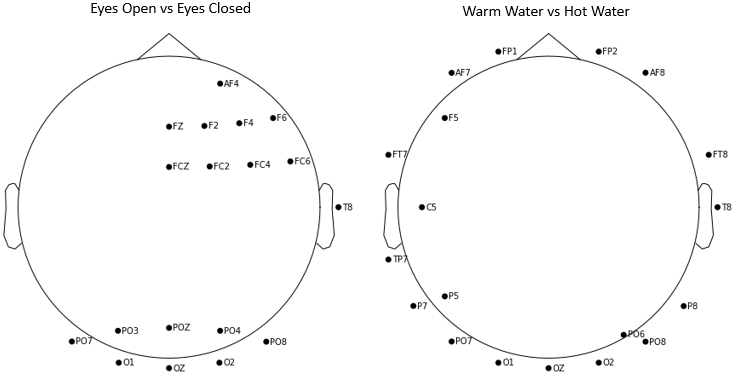
\includegraphics[width=0.95\textwidth]{ROI.png}
\caption{\label{fig:ROI}
Scalp topographies depicting the general regions of interest for both occular activites and water emersion respectively. These optimal channels were calculated by finding the power spectral densities in each frequency band with the highest differences for two given experimental events. Although the patterns seem fairly arbitrary, there are some useful characteristics that confirm intitial feature analyis, such as a occipital lobe biased channel selection.}
\end{figure} 

At first the distribution of channels seem fairly arbitrary. However upon further inspection we can see patterns correlating to the event analysis undertaken in the previous chapter. For example, earlier in the article we concluded that occular activity tends to originate primarily from the occipital region of the scalp. The ROI topographies seemingly confirm this. We can also see a fairly intentional pattern in the frontal portion of the scalp. The region of interest topography for the pain stimuli is fairly comparable to that of the occular activities; a strong distribution between the frontal and occipital portions of the scalp. Although there are no immediate articles in the literature that can corroborate this distribution, we can assume that it is fairly accurate given the high accuracies achieved by our final models.

\section{Data Classification}

Label classification has been evaluated using three different approaches. Although each of these algorithms work in a unique fashion, they are designed to operate with the same output; to find the best combination of channels for a specific classification problem. These feature selection algorithms have been discussed in more detail below. Given that our approach involves using a chain of estimators it seems fitting to invoke a pipeline that will sequentially apply our required transformations as well as a final estimator. The final estimator in our case will be the support vector machine \cite{cortes1995support}. SVMs are one of the most common and well-performing models in signal classification. There is a vast selection of literature proven scenarios in which this model has performed impressively well, alot of which have been cited in this article. 

Support vector machines work by seperating our labelled training data onto a plane and plotting a hyperplane that best seperates them based on their labels. The hyperplane, is often also referred to as the decision boundary. Support vector machines consider the best hyperplane the one that maximises the margins from all the labels in the classification problem. Typically SVMs perform extremely well when faced with high dimensional feature spaces, naturally making it one of the best choices for this project. Another benefit of support vector machine come from it's ability to invoke multiple kernals. Each kernal can be applied to buffer the mean accuracy of any model output. That being said due to unfortunate time constraints, only the linear kernel was tested against our training data.

\subsection{Common Spatial Patterns}

Common spatial patterns are one of the first feature selection algorithms used in combination with our base classifier, the support vector machine \cite{4634130}. The goal of this algorithm is to use spatial filters to maximise the distinguishability between two experimental events or classes. Over the last few years, the common spatial pattern algorithm has been predominantly used to decode motor imagery and was found to be extremely effective on multiple occasions. Motor imagery is a mental process of a motor action. Motor imagery is usually measured in combination with a brain machine interface which acts as a direct pathway between the brain and an external device. In 2018, Carlos Gonzalez was able to classify motor imagery eeg signals using CSP filtering in combination with various deep neural networks to an accuracy of up to 89\% \cite{CSP}. Common spatial patterns are designed to thrive in noisy environments and cater to cases in which over fitting the data may be more prominent. Given the nature of our input data prone to containing noisy components, this algorithm was predicted to perform the most effectively during the classification stages of the article.

When providing the data to our classification models, we use the combined outputs from 63 channels worth of power spectral densities. Most of these channels will contain features that are completely useless when classifying between two experimental events. The goal of the CSP algorithm is to produce a linear combination of channels which vary the most with respect to our labelled data. Similarly to the feature anaylsis undertaken previously, we are trying to find which combination of channels have the most useful information contained for classifying our pain states, and which ones contain data that is just inflating our feature dimensions and lowering the potential accuracy of the model. Note that common spatial patterns is a data driven algorithm and it's highly possible that subtly different datasets will not cause the algorithm to converge on a reasonable combination of useful channels. That being said, the effectiveness of the model should be easy to spot via it's final mean accuracy. 

The cross validation technique used in combination with CSP and SVM is k-fold cross validation \cite{CV}. This technique splits the data into k folds (in our case 10), of which the first 9 are used for training, and the final fold used for testing. This is then shuffled and repeated k times until each unique fold has been used for both training and testing. K-fold cross validaton works most optimally for balanced datasets which is why stratified k-fold has been utilized as opposed to the normal algorithm. Stratification is an extension of the cross-validation technique and works by mainting the ratio of class labels between two classes during each fold. Given this articles implementaton boasts ten folds, our final accuracy is defined as the mean accuracy of each of the ten folds. 


\subsection{SPoC}

SPoC, source power comodulation, is the second feature selection algorithm used for our signal classification. SPoC, differently to other feature selection algorithms, focuses on the power dynamic of oscillatory sources. It works by attempting to isolate the components of the training data who's power best comodulates with that of the target variable. SPoC, similarly to common spatial patterns essentially produces a linear combination of channels that contain the most promising data for classifying our pain states. First introduced in 2015, Sven Dahne et al. were able to introduce the novel approach to SPoC whereby two algorithms could be used to implement it's functionality \cite{DAHNE2014111}. By extracting "neuronal components exhibiting high correlation of power with the target variable", they were able to prove that the algorithm outperforms a range of commonly used techniques that utilize sensor data. Often SPoC is regarded as an extension of common spatial patterns with the difference being driven by a continuous variable as opposed to a discrete variable. SPoC has been implemented using the same pipeline as the CSP algorithm however using regular k fold as opposed to stratified k fold. Given our dataset was epoched using the same number of trials for each experimental event, we can consider ratio of class labels in the training data balanced. Our final accuracy is defined as the percentage of correct label predictions for our testing split.


\subsection{Riemannian Classifier}

The riemannian classifier, whilst recently increasing in popularity, is beginning to demonstrate a plethora of promising articles that successfuly classify electroencephalogram signals and outperform the conventional spatial filtering methods \cite{Riemannian}. Riemannian classification as opposed to spatial filtering or feature selection, works by mapping data directly onto a geometrical space in combination with a suitable metric. Once the data is mapped into the geometrical spaced, it can be classified using two methods: local and linear approximation. Similar to the previous classification models, riemannian classification has been implemented via a pipeline of different transformations, followed by our final estimator, which in this case is the support vector machine. 

We initialize our pipeline by computing the covariance matrix of our inputs. A covariance matrix is essentially a symmetrical representation that demonstrates the covariances between a set of values. There are multiple metrics available, however commonly they represent the distribution magnitude and direction of multivariate data in a multidimensional space. Using a covariance matrix, we can obtain information about how spread out our features are given a set of dimensions. Below is an example of the covariance formula used to calculate the covariances between a vector of values from an input dataset.

\begin{gather}\label{eq:1.1}
cov_{x,y}=\frac{\sum_{i=1}^{N}(x_{i}-\bar{x})(y_{i}-\bar{y})}{N-1}
\intertext{Where:}
\begin{aligned}
&cov_{x,y} \text{ = Covariance between variable {x} and {y}}\\
&x_{i} \text{ = Value of {x}}\\
&y_{i} \text{ = Value of {y}}\\
&\bar{x} \text{ = Mean of {x}}\\
&\bar{y} \text{ = Mean of {y}}\\
&N \text{ = Number of data values}
\end{aligned}\notag
\end{gather}

Once our covariance matrix has been computed, we need to transform our data to the tangent space. The process of tangent space projection maps a set of matrices to their tangent space using a unique kernal operation resulting in matrices represented as a series of vectors. The transformation aims to conserve the inner structure of the manifold whilst transforming the data into a series of euclidean vectors for which the conventional vector-based classification can be applied. Given the three transformations required in the pipeline, the time taken to train our Riemmanian based model, is significantly longer than common spatial patterns and source power comodulation. 

Although there hasn't been any obvious articles published that investigate the classification of pain states using Riemmanian geometry, there is an abundnace of literature demonstrating the effectiveness of the procedure when exposed to brain signals sourced from human motor imagery. In 2020, Abu Saleh Musa Miah et al. investigated how a unique approach to riemmanian geometry using median absolute deviation would be able to classify motor imagery EEG data \cite{RIE}. The conclusion made from this article was that the proposed method was able to outperform a host of other sophisticated classification methods, including that of common spatial patterns and linear discriminant analysis. Riemannian geometry was measured to be approximately 90.33\% accurate when predicting the testing data's labels; the highest performing model in the entire article. Similarly to common spatial patterns, the cross validation procedure invoked in this pipeline was stratified k-fold, ensuring that the ratio of class labels stayed constant when the folds were computed.


\section{Results}

\begin{center}
  \begin{tabular}{ccccccc}
    \hline
    \multirow{2}{*}{Dataset} &
      \multicolumn{3}{c}{Eyes Open vs Eyes Closed} &
      \multicolumn{3}{c}{Warm Water vs Hot Water} \\
    & CSP & Riemannian & SPoC & CSP & Riemannian & SPoC \\
    \hline
    3TM\_01-100 & 93.3 & 100 & 85.7 & 100 & 100 & 100 \\
    4EB\_01-100 & 100 & 100 & 87.6 & 85.0 & 98.6 & 74.0  \\
    5LL\_01-100 & 100 & 100 & 80.0 & 83.3 & 95.6 & 70.0 \\
    7IG\_01-100 & 100 & 100 & 80.0 & 88.6 & 95.7 & 67.6 \\
    10OS\_01-100 & 93.3 & 95.0 & 79.3 & 84.5 & 97.1 & 86.4 \\
    11TP\_01-100 & 96.7 & 100 & 86.2 & 90.2 & 98.6 & 90.1 \\
    13MT\_01-100 & 100 & 100 & 85.7 & 96.9 & 100 & 96.9 \\
    14JR\_01-100 & 95.0 & 96.7 & 71.4 & 80.2 & 98.6 & 62.5 \\
    15DM\_01-100 & 100 & 100 & 96.7 & 85.5 & 100 & 81.2 \\
    16ET\_01-100 & 83.3 & 100 & 85.7 & 80.4 & 100 & 76.3 \\
    17RP\_01-100 & 96.7 & 96.7 & 86.7 & 96.5 & 100 & 75.9 \\
    18EB\_01-100 & 100 & 96.7 & 96.6 & 76.2 & 97.5 & 76.2 \\ 
    19HB\_01-100 & 96.7 & 100 & 95.7 & 100 & 100 & 100 \\
    20JC\_01-100 & 83.3 & 96.7 & 66.7 & 98.9 & 100 & 87.5 \\
    22NL\_01-100 & 100 & 100 & 83.3 & 90.2 & 100 & 82.2 \\
    25DE\_01-100 & 93.3 & 100 & 86.2 & 88.8 & 92.3 & 66.7 \\
    27KA\_01-100 & 93.3 & 96.7 & 89.7 & 43.9 & 96.7 & 56.9 \\
    28KC\_01-100 & 95.0 & 100 & 100 & 62.8 & 97.8 & 70.9 \\
    30CK\_01-100 & 100 & 100 & 93.1 & 88.1 & 98.6 & 83.8 \\
    31JV\_01-100 & 86.7 & 100 & 85.7 & 76.5 & 94.3 & 56.9 \\
    32AC\_01-100 & 93.3 & 100 & 75.0 & 64.6 & 94.9 & 58.3 \\
    33IG\_01-100 & 96.7 & 100 & 96.6 & 90.0 & 98.6 & 77.1 \\
    34GL\_01-100 & 88.3 & 100 & 75.0 & 69.3 & 94.6 & 64.9 \\
    35JH\_01-100 & 100 & 100 & 93.1 & 55.4 & 96.7 & 68.5 \\ 
    36MS\_01-100 & 86.7 & 96.7 & 93.1 & 79.2 & 96.0 & 75.2 \\
    37DG\_01-100 & 76.7 & 100 & 73.3 & 78.0 & 97.9 & 60.4 \\
    38JC\_01-100 & 91.7 & 100 & 75.9 & 76.7 & 97.1 & 61.8 \\
    39MF\_01-100 & 90.0 & 100 & 82.8 & 91.4 & 95.9 & 87.7 \\
    40SL\_01-100 & 100 & 100 & 100 & 89.2 & 98.8 & 80.2 \\
    41IA\_01-100 & 96.7 & 96.7 & 86.2 & 95.0 & 95.0 & 57.1 \\
    \hline
    Mean Accuracy & 94.2\% &\textbf{99.1\%} & 85.7\% & 81.8\% & \textbf{97.6\%} & 75.1\% \\
    STD & \textpm 0.06 & \textpm 0.02 & \textpm 0.09 & \textpm 0.14 & \textpm 0.02 & \textpm 0.13 \\
    \hline
  \end{tabular}
\end{center}


The purpose of this study was to ascertain to what degree we could classify simulated pain states in participants using tailored machine learning pipelines. It further examines what regions of the scalp emit the brain signals responsible for our high accuracy classification. By displaying our classification results across all models and datasets in tabular form, we can see an impressive mean accuracy for each model. It should be noted that classifying our eyes open and eyes closed experimental events is just a test for our models to evaluate their initial performances. Due to the subtle difference between emersion events, if the classification score for our occular activity, where the difference is not so subtle, was low, it would be clear that our models would not be able to handle the classification of warm water and hot water emersion. This would indicate further improvements would have to be made to either the preprocessing stages of the pipeline, or the models themselves. However we can see that across all datasets, common spatial patterns, Riemannian classification and the source power comodulation algorithm have performed exceedingly well with mean accuracies of 94.2\%, 99.1\% and 85.7\% respectively. Given the difficulty of classifying two extremely similar signals, our models were able to distinguish between hot water and warm water emersion extremely successfuly. Both the common spatial pattern and source power comodulation pipelines were able to predict pain states with mean accuracies of 81.8\% and 75.1\% respectively. That being said the Riemanninan classifier, similar to the occular experimental events, was able to outperform both the spatial filtering methods with a mean accuracy of 97.6\% and a standard deviation of \textpm 0.02. Multiple reruns of the source code were undertaken to verify the validity of these results, with each resulting in a very similar value. These results confirm that the Riemannian classifier, being the newest model of the three, is the best performing model with regards to signal classification.

\section{Discussion}

Although mean accuracy is a useful metric for evaluating how well our models can predict event labels, it's imperative that we investigate whereabouts our feature selectors extrapolated their most useful data from. There are two main categories that can be explored that demonstrate what factors contribute the most to our models, these being the regions of the scalp emitting the most useful brain signals, and the best performing frequency ranges inside the signal. Note that knowing the best performing frequency ranges, allows the plotting of regions of interest with respect to each frequency band as well. Unfortunately, pyRiemann does not offer any immediate analysis plots that allow for the above objectives. That being said, given the sufficiently high accuracy of our common spatial patterns pipelines, it could be argued that viewing the plots produced by these models would be sufficient. 

\subsection{Regions of Interest}

The first region of interest evaluations are conducted over the 1-40Hz signal range. It should be noted that due to an arbitrary concentration of weights around the electrodes PO5, PO6 and M2, these channels were removed from our topographies and resulted in a much more balanced distribution. Electrode flaws of this nature can be caused by a number of different issues the most likely being a poor connection between an electrode and the scalp. Initial inspections of the scalp topographies for the warm water and hot water emersion indicated no major patterns with regards to the weight distribution. For most of the plots, the distribution seemed fairly arbitrary with the models selecting channels from all regions of the scalp \ref{fig:3TM_WW}. That being said, there were a few cases in which channels selected were primarily from the occipital and frontal region of the scalp which lines up with the feature analysis undertaken previously in this article. Were this kind of pipeline deployed into a real medical environment, the result obtained from our models would be more than sufficient to adequately detect pain states in patients with conditions that make communication difficult. 

\begin{figure}[tb]
\centering
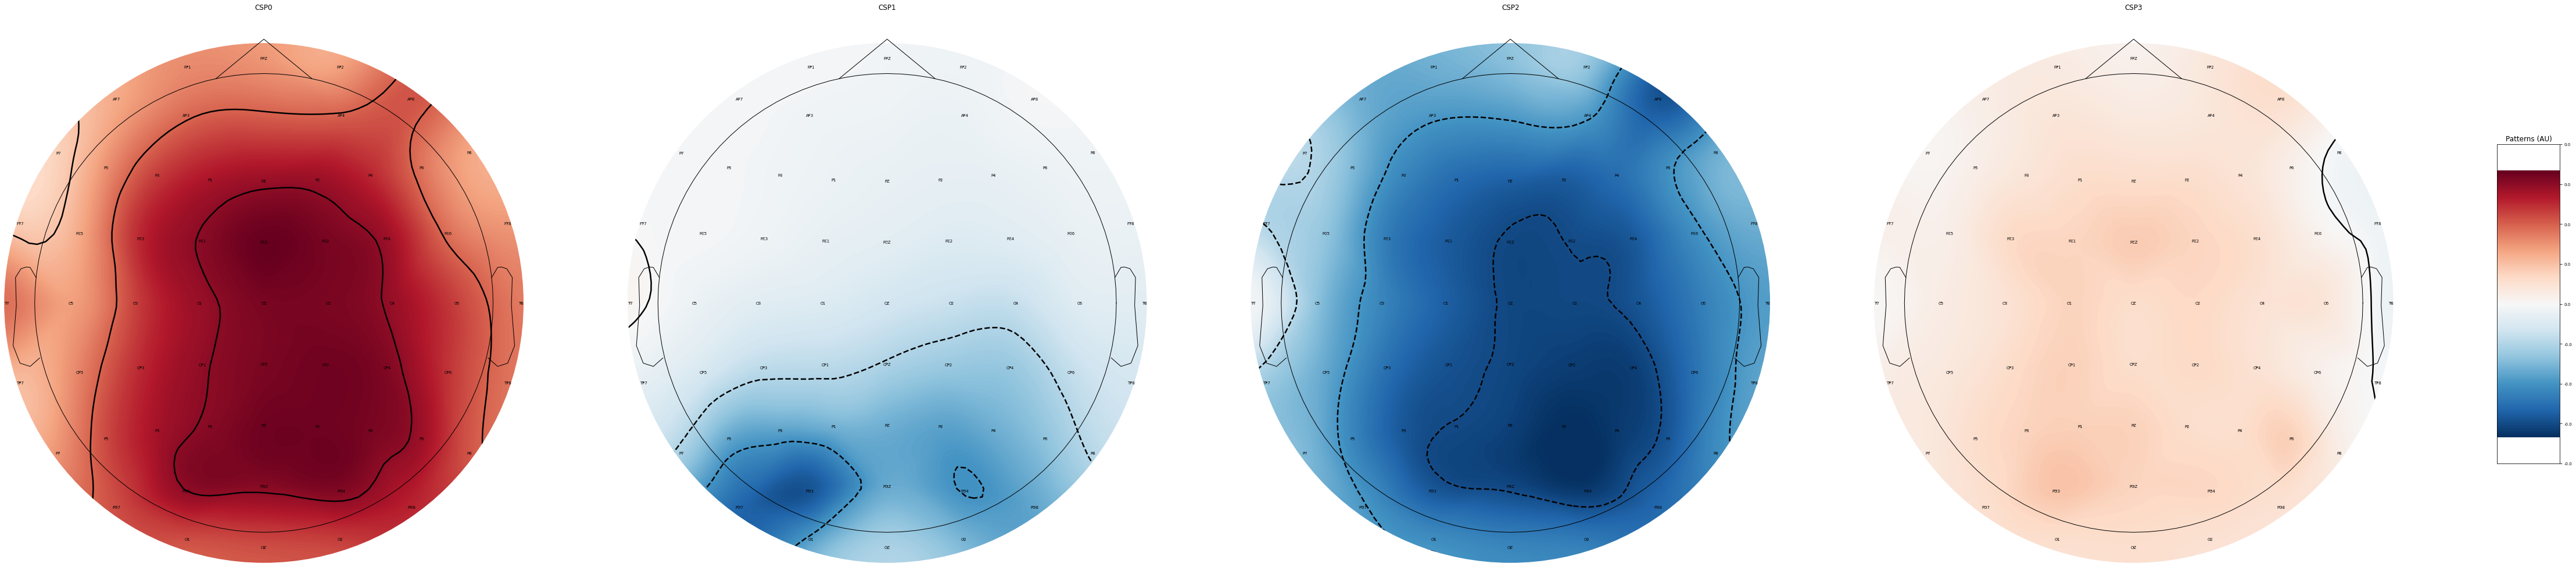
\includegraphics[width=0.95\textwidth]{3TM_WW.png}
\caption{\label{fig:3TM_WW}
Scalp topography depicting the channels selected by common spatial patterns for pain state classification. Throughout all datasets, the scalp topographies demonstrated a fairly arbitrary weight distribution with the algorithm selecting channels from all regions of the scalp. In some cases the distribution was more prominent in the frontal and occipital regions.These topographies were plotted using the results of dataset 3TM; the dataset with the highest recorded model accuracies.}
\end{figure} 

\subsection{Regions of Interest by Frequency Band}

By calculating our power spectral densities with respect to specific frequency ranges, we are able investigate which frequency bands contribute the most to our model's accuracies. Note that the table below displays the results of the Riemannian classifier only due to the consistent outperforming of it's spatial filtering counterparts.

\begin{center}
  \begin{tabular}{cccccc}
    \hline
    \multirow{2}{*}{Metrics} &
      \multicolumn{5}{c}{Warm Water vs Hot Water} \\
    & Delta & Theta & Alpha & Beta & Gamma \\
    \hline
    Mean Accuracy & 77.4\%  & 72.5\%  & 73.1\%  & \textbf{91.4\%}  & \textbf{89.2\%} \\
    Standard Deviation & \textpm 0.09  & \textpm 0.11  & \textpm 0.10 & \textpm 0.08  & \textpm 0.09 \\
    \hline
  \end{tabular}
\end{center}

The best performing frequency bands for classifying between hot and warm water emersion are the 12-30Hz (Beta) and 35Hz+ (Gamma) ranges with mean accuracies of 91.4\% and 89.2\% respectively. Current literature regarding the most influencial frequency ranges for classifying pain states are fairly varied. For example, Mingxin Yu et al. managed to classify tonic pain using neural networks and found the Alpha and Beta bands to be the best performing frequency ranges \cite{YU2020270} whereas Gaurav Misra et al. when classifying thermally induced pain found the Beta, Gamma and Theta bands to be the best performing \cite{Misra2017-ol}. Given conclusions made in a range of previous articles, there does seem to be a fairly reoccuring pattern, with both the Beta and Gamma bands consistently demonstrating their benefit for classifying between pain and non-pain states. Furthermore, these results confirm the observations made earlier in the article during warm water vs hot water event analysis, where obscure patterns could be distinguised between the Beta and Gamma sections of the line graphs \ref{fig:Chart_Pain}. By utilizing the same technique as before and plotting the common spatial pattern scalp topographies for each frequency band, we can observe the most influential regions of interest \ref{fig:All}. 

\begin{figure}
     \centering
     \begin{subfigure}[b]{1\textwidth}
         \centering
         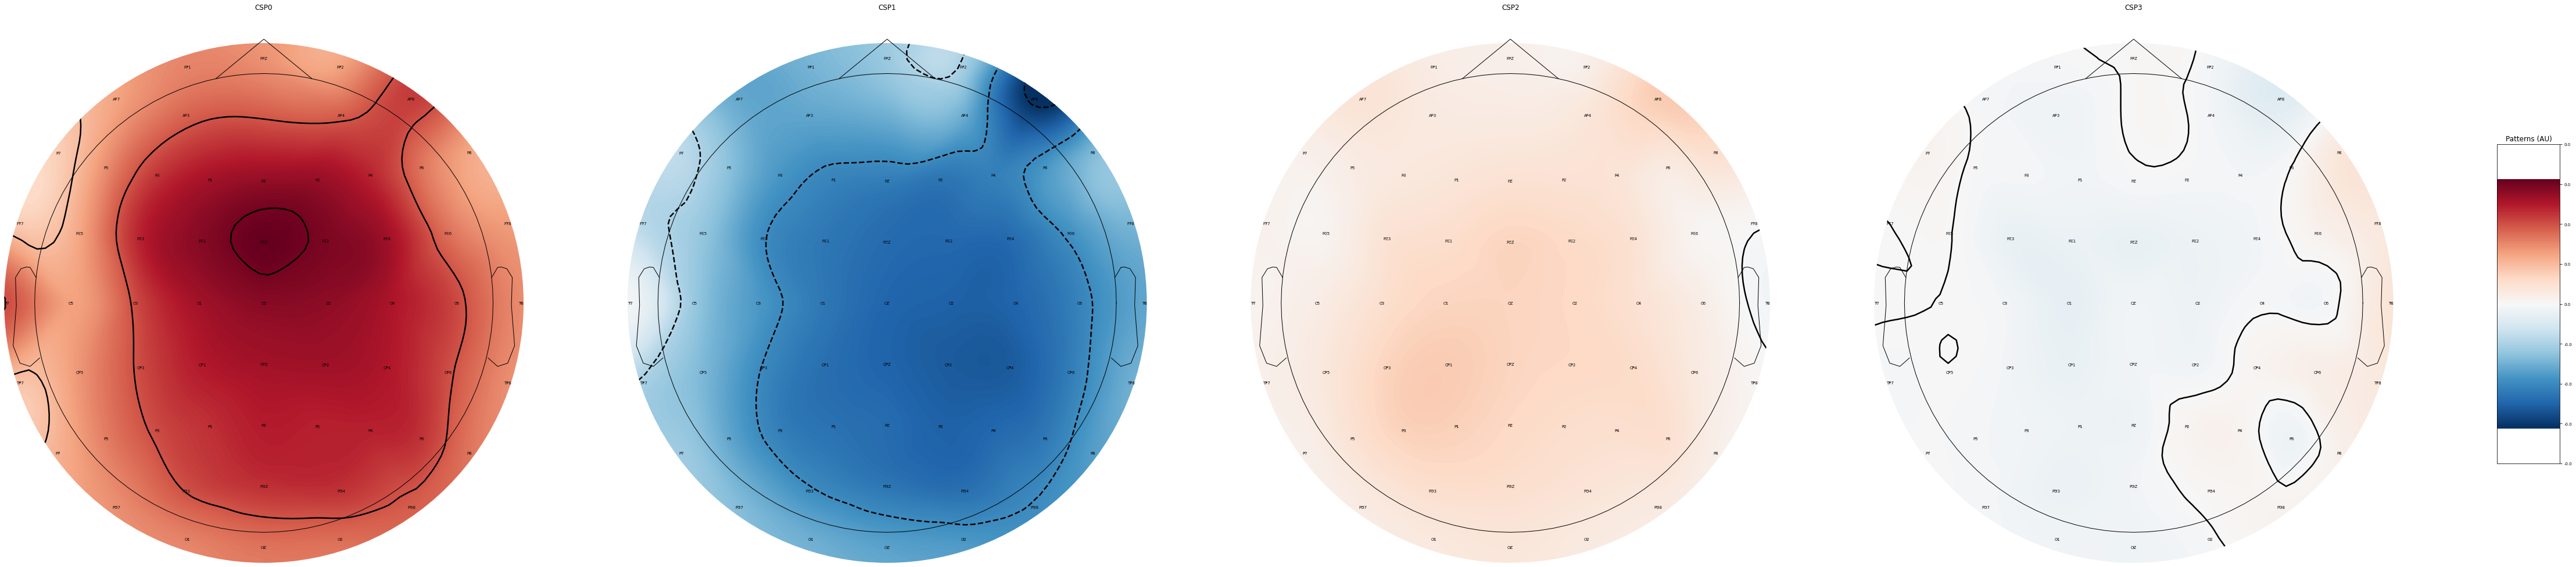
\includegraphics[width=\textwidth]{Delta_Top.png}
         \caption{Delta Range Only}
         \label{fig:Delta}
     \end{subfigure}
     \hfill
     \begin{subfigure}[b]{1\textwidth}
         \centering
         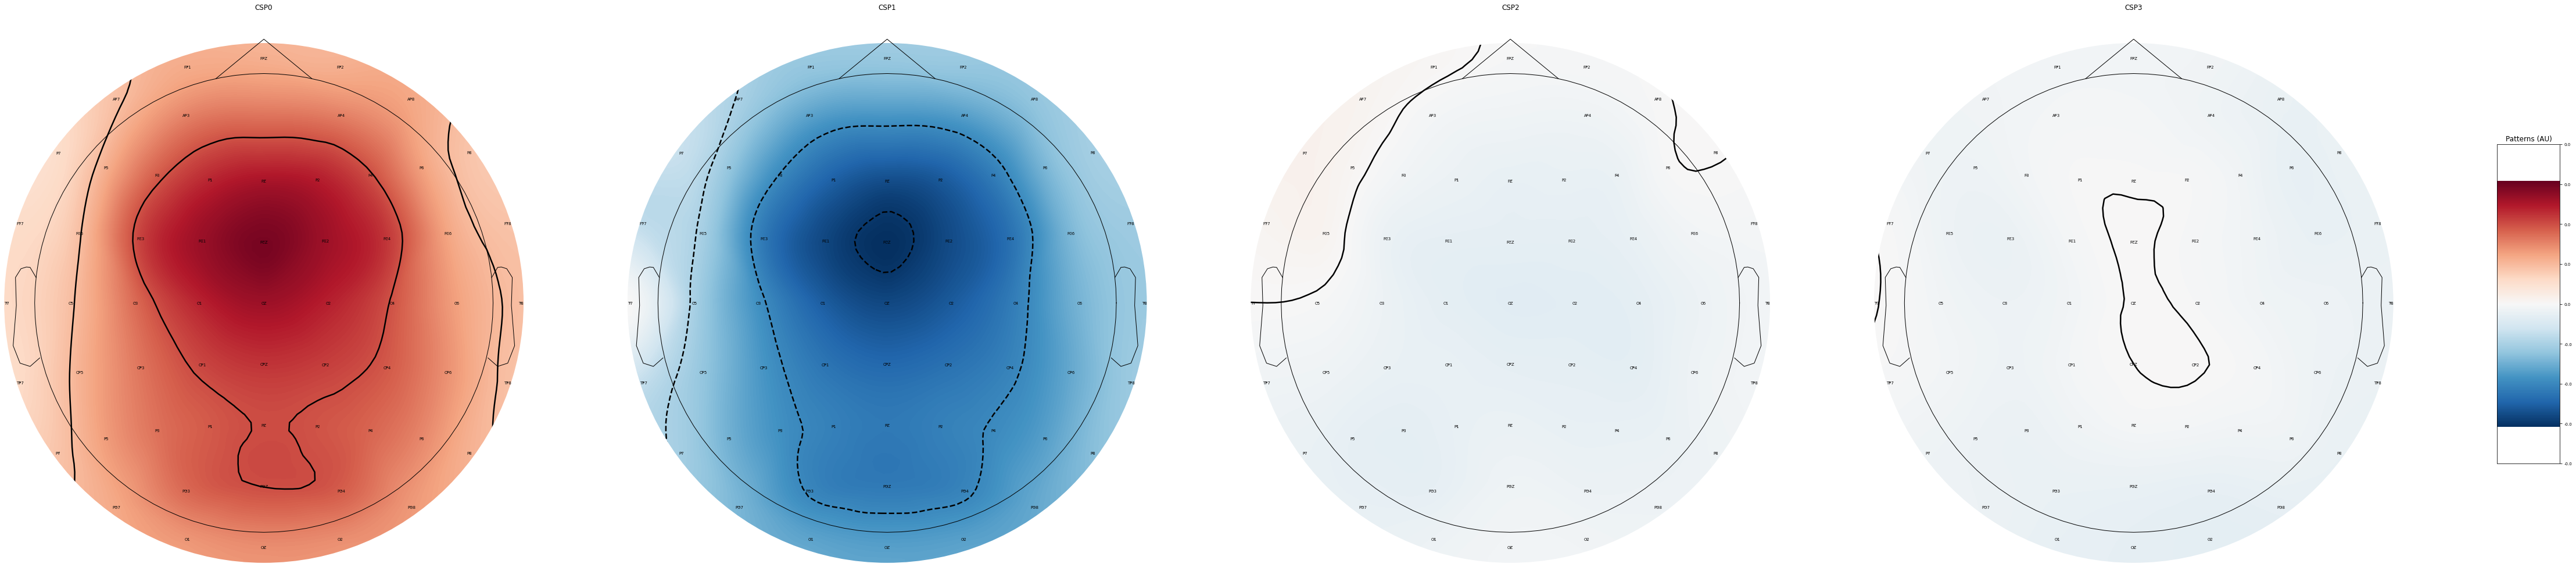
\includegraphics[width=\textwidth]{Theta_Top.png}
         \caption{Theta Range Only}
         \label{fig:Theta}
     \end{subfigure}
     \hfill
     \begin{subfigure}[b]{1\textwidth}
         \centering
         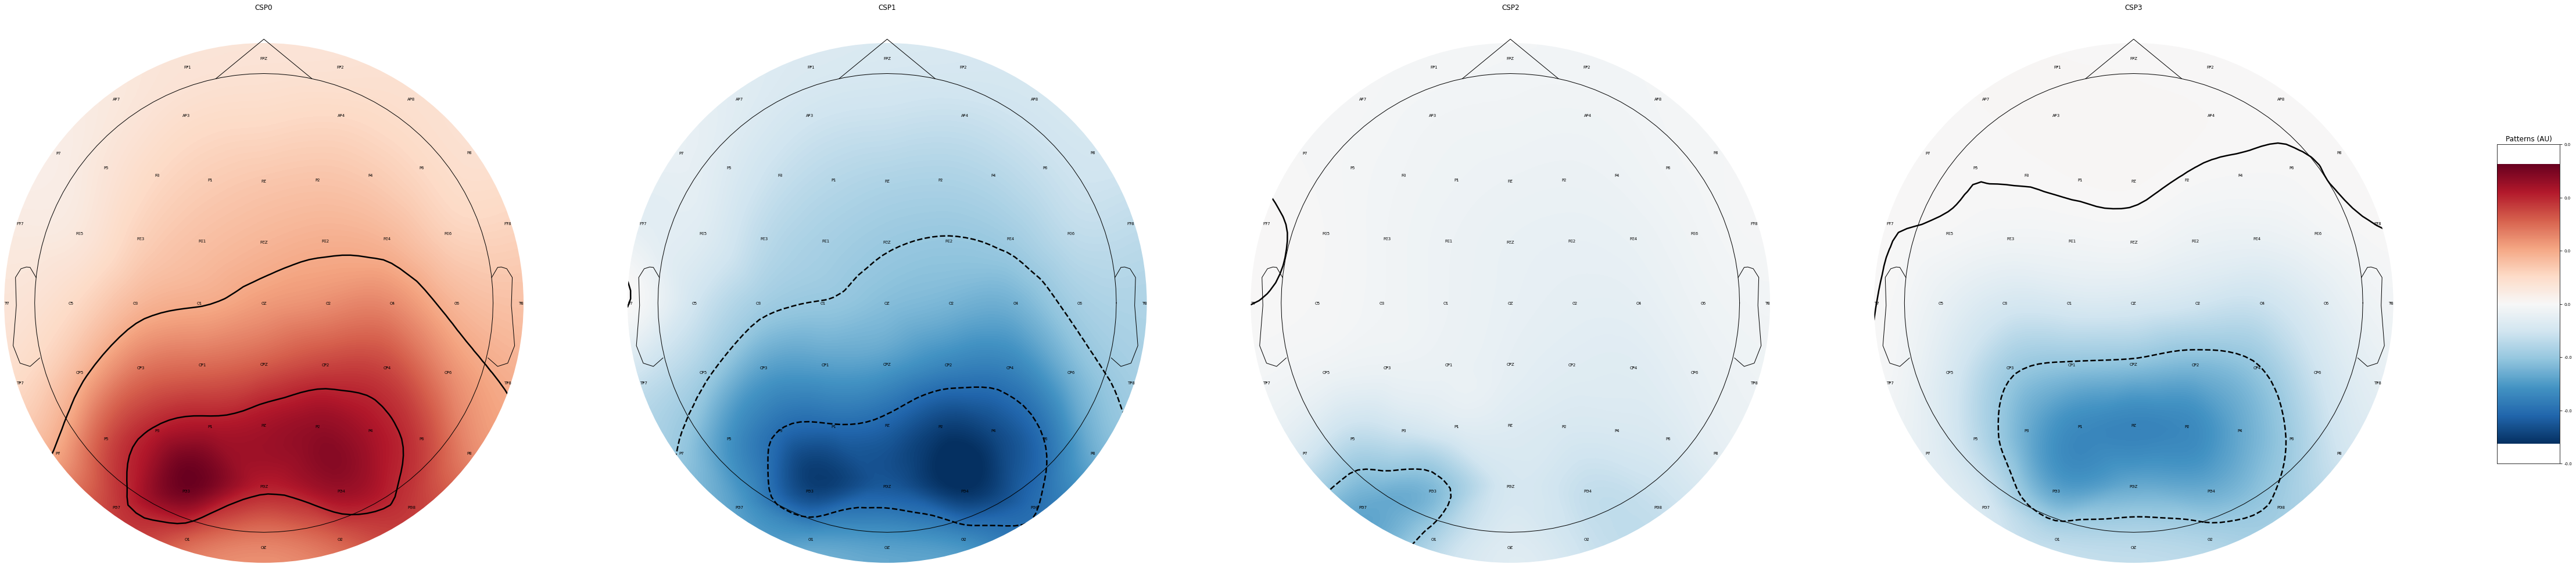
\includegraphics[width=\textwidth]{Alpha_Top.png}
         \caption{Alpha Range Only}
         \label{fig:Alpha}
     \end{subfigure}
     \hfill
     \begin{subfigure}[b]{1\textwidth}
         \centering
         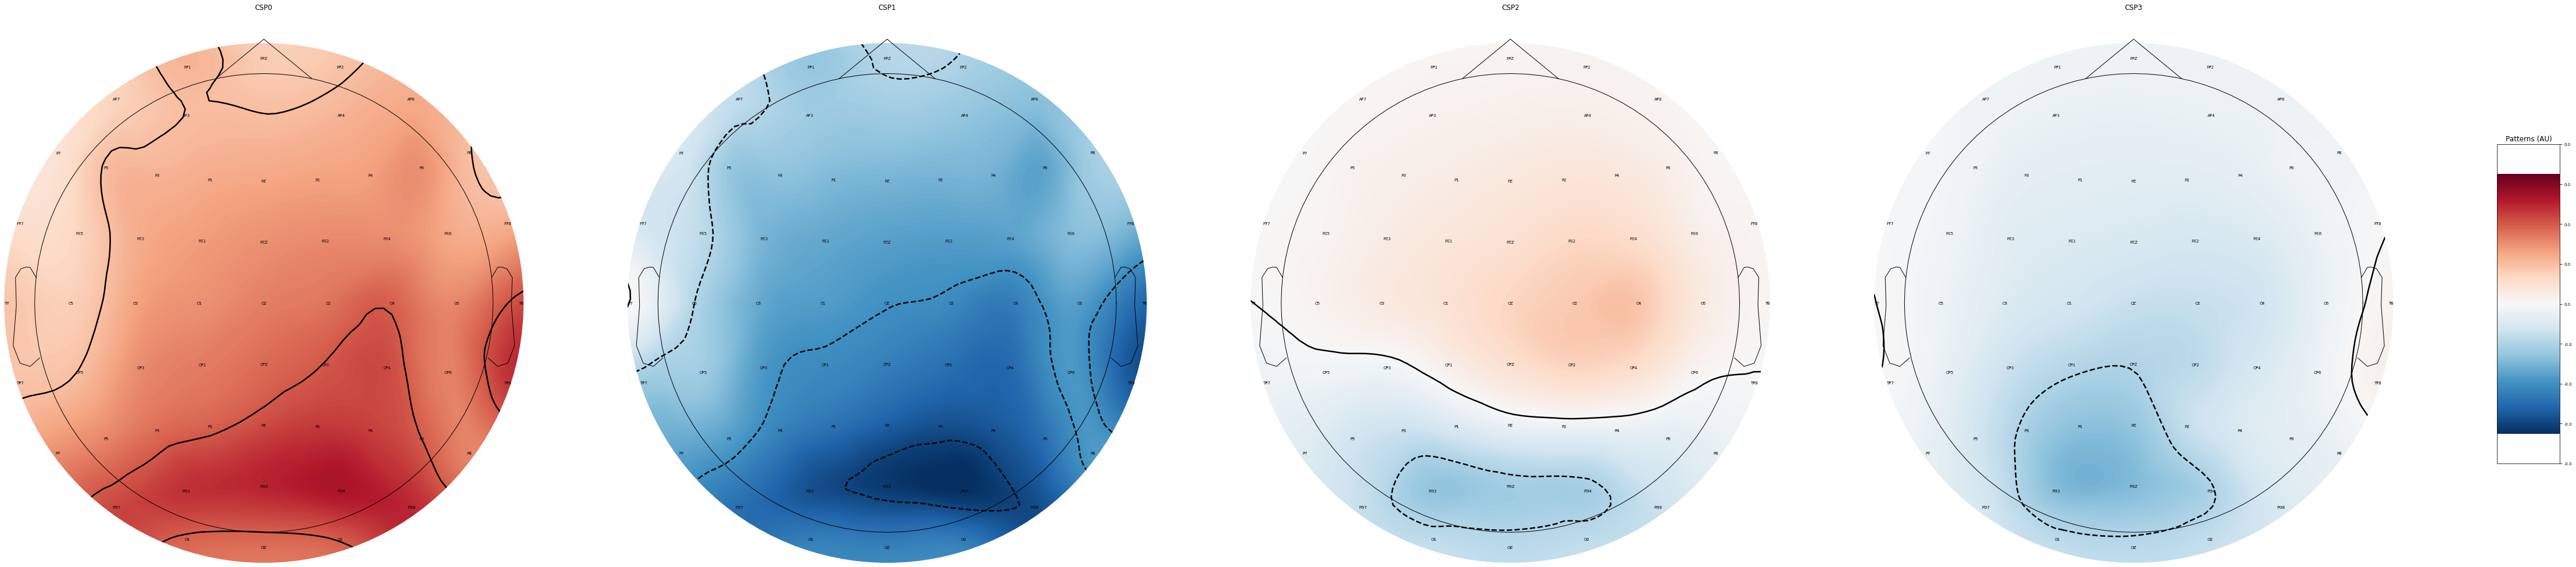
\includegraphics[width=\textwidth]{Beta_Top.png}
         \caption{Beta Range Only}
         \label{fig:Beta}
     \end{subfigure}
     \hfill
     \begin{subfigure}[b]{1\textwidth}
         \centering
         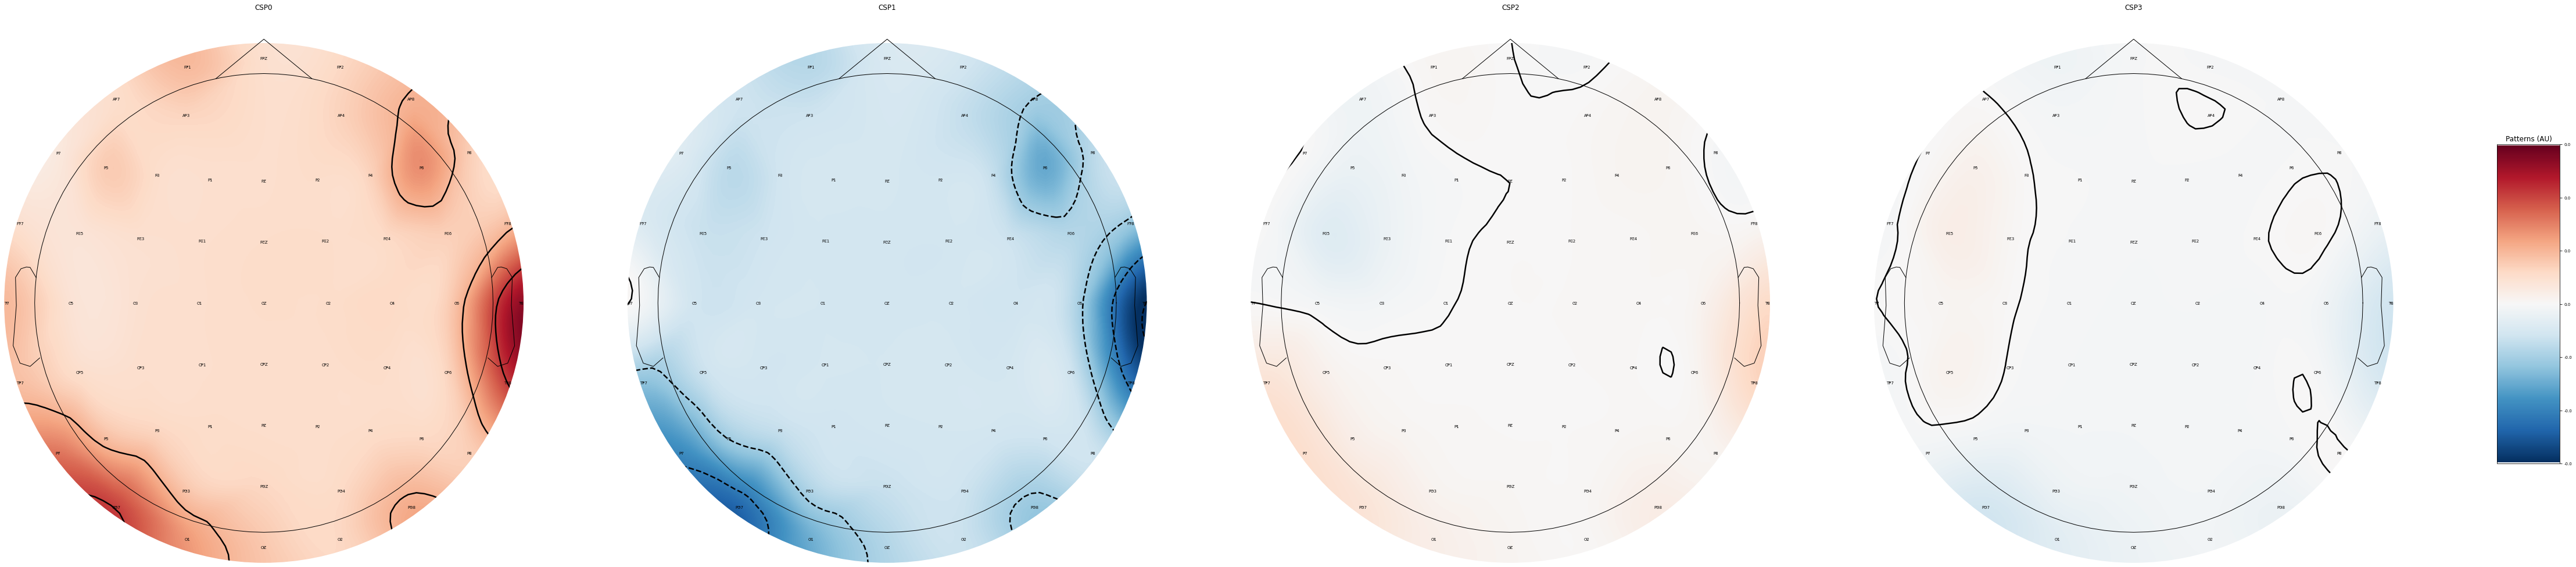
\includegraphics[width=\textwidth]{Gamma_Top.png}
         \caption{Gamma Range Only}
         \label{fig:Gamma}
     \end{subfigure}
        \caption{Scalp topographies depicting the channels selected by common spatial patterns for warm water vs hot water emersion. Each of the figures were recorded under their respective frequency band constraints. Most of the figures from each range demonstrated similar characteristics across all datasets. These topographies were plotted using the results of dataset 3TM; the dataset with the highest recorded model accuracies.}
        \label{fig:All}
\end{figure}

Inspections of the five sets of scalp topographies indicate 3 different patterns. For both the delta and theta frequency ranges, there seems to be a predominantly central distribution of weights at the vertex of the scalp. On the other hand, the Alpha and Beta ranges seem to have selected channels more towards the occipital region of the scalp. Using previous literature, we can confirm a fairly confident pattern with the Beta frequency range associating the most with the occipital region of the scalp. That being said there are widely popular articles that contradict these findings \cite{Misra2017-ol}. For example, Gaurav Misra et al. stated in their discussion that the significant decrease in Beta power that lead to their high classification accuracies originated from the contralateral sensorimotor cortex, which is more towards the central part of the scalp as opposed to the occipital region. 

The gamma frequency range seems to indicate a fairly unorthadox pattern with there being two strong weight congregations; one on the right temporal portion of the scalp, and the other at the left occipital region of the scalp. Gaurav Misra et al. when analysing feature dependencies noticed their increase Gamma originating predominantly from the medial prefrontal cortex at the front of the scalp which starkly contradicts the findings of our topography. It could be argued that electrode flaws could be the root cause of this difference. That being said, the classification of pain states is fairly sparsely investigated so neither conclusion can be confirmed. Either way it's clear that both Gamma and Beta are the best frequency ranges to utilize when classifying between pain and non-pain states. 
\subsection{Further Work}

Although the results of riemannian classifer demonstrate effective predictions for simulated pain states, there are major components to the project that could be extended to improve the general quality of the pipeline. The first is the introduction of the automatic artifact retrieval toolbox. One of the pipelines underlying drawbacks, is it's requirement to manually perform independant component analysis on each dataset. The process is extremely time consuming and can amount to several extra hours of work for thos with large datasets. The AAR toolbox bases it's methods on regression techniques and adaptive algorithms such as least mean squares (LMS) and recursive least squares (RLS) in combination with blind source seperation to automatically decompose the signal. Having the ability to remove artifacts based on a set criteria will make the pipeline infinitely more automated and reduce the possibility of human error during the artifact detection process.

The second is the interpolation of purposely removed channels. As stated previously in the article, the channels T7, PO5, PO6 and M2 were removed due to their arbitrary skewing of the classification and analysis results. Instead of removing these channels outright, it would be more optimal to interpolate the values of these channels to their nearest neighbour, simulating a more balanced distribution of frequencies across the signal. MNE offers two different methods to interpolate "bad" EEG channels the most common of the two being spherical splines for evoked objects. 

The final improvement to be made on the pipeline, is the reduction in epoch segmentation time. When the data is been epoched into it's experimental events, the epochs need to be epoched again into equal length trials, each of which represent a single row in our training dataframe. The time interval at which each epoch was segmented, was set to 10 seconds. Given the length of our experiments results, an average of 43 trials for our pain states were taken. Fourty three trials can be argued as insufficient for our training data. A subtle decrease to 7 second intervals would result in a significantly larger number of trials giving our classification models sufficient data to train with.



\bibliographystyle{abbrv}
\bibliography{Citations_File}

\end{document}